\chapter{Set Theory}%!chapter

\section{Sets and Elements}
\begin{definition}
    A set is a well defined list or correction of objects.
\end{definition}

\begin{definition}
    An object that belongs to a particular set is called an element or a member of that set.
\end{definition}

\section{Set Notations:}

\begin{para}
    Uppercase letters of the alphabet, i.e., $A, B, M, X$ are used to denote sets an lowercase letters i.e., $a, b, m, x$ for members of sets
\end{para}

\begin{para}
    if $A$ is a set and $k$ its element, then the expression $k \in A$ is read as "$k$is an element of $A$". If $p$ is not a member of $A$ it is written as $p \notin A$
\end{para}

\subsection{Examples of Sets}

\begin{para}
    To specify that certain objects belong to a given set, the braces, \{\} called set builders are used by either providing a \underline{roster} i.e., complete list of all elements in the braces or the \underline{rule} method i.e., stating properties that characterize the elements within the braces
\end{para}

\begin{examples}
    \mbox{}\\[-\baselineskip] %empty line
    \begin{enumerate}
        \item $A = \{1,2,3,5,7,11\}$ means is a set consisting of numbers $1,2,3,5,7,$ and $11$
        \item $B = \{x:$ x is a prime number; $x < 13\}$ means $B$ is a set of prime numbers less than $13$
        \item $17 \notin A$ means $17$ is not a member of set $A$
    \end{enumerate}
\end{examples}

\section{Subset}

\begin{definition}
    Let $A$ and $B$ be two sets. If every element of $A$ also belongs to $B$ i.e, if $p \in A \implies p \in B$,then $A$ is called a subset of $B$ or is said to be contained in $B$.
\end{definition}

\begin{para}
    Two different types of subsets emerge from this definition of subset: \underline{proper} and \underline{improper} subsets.
\end{para}

\begin{definition}
    A is a proper subset of $B$, if it is a subset of $B$ and there exists at least one element of $B$ that does not belong to $A$. Otherwise $A$ is an improper subset of $B$.
\end{definition}

\section{Subset Notation}

\begin{para}
    To show that $A$ is a subset of $B$ we write it as $A \subset B$.
\end{para}

\subsection{Subset Examples}

let
$\mathbb{N} = \{1, 2, 3, \ldots\}$\\
$\mathbb{Z} = \{\ldots, -2, -1, 0, 1, 2, \ldots\}$\\
$\mathbb{R} = \{x: \text{ x is a real number}\}$\\

Then $\mathbb{N} \subset \mathbb{Z} \subset \mathbb{R}$

\begin{para}
    A subset of real numbers can also be defined as an interval on the real line

    \begin{center}
        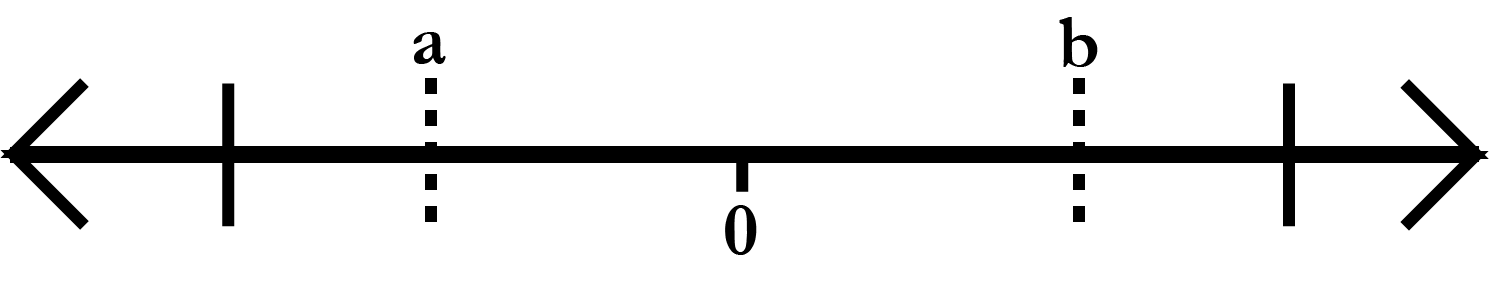
\includegraphics[width=0.3\linewidth]{chapter/sets and elements/numberLine.png}
    \end{center}

\end{para}


\begin{examples}
    \mbox{}\\[-\baselineskip] %empty line
    \begin{enumerate}
        \item $(a,b) = \{x:  a<x<b\; x \in \mathbb{R}$\\
              means an open interval of real numbers from $a$ to $b$.
        \item $[a,b] = \{x: a \leq x \leq b; x \in \mathbb{R}\} $\\
              means $a$ closed interval of real numbers from $a$ to $b$.
        \item $(a,b] = \{x: a < x \leq b; x \in \mathbb{R}\} $\\
              means an open-closed interval of real numbers from $a$ to $b$.
        \item $[a,b) = \{x: a \leq x < b; x \in \mathbb{R}\} $\\
              means an closed-open interval of real numbers from $a$ to $b$.
    \end{enumerate}
\end{examples}
\section{Equal Sets}
\begin{definition}
    Two sets are equal if each set is contained in another i.e., let $A$ and $B$ be any two sets, then if $x \in A \implies x \in B$ and $x \in B \implies x \in A$, we have $A = B$
\end{definition}

\begin{para}
    In other words $A=B$ if and only if $A \subset B$ and $B \subset A$
\end{para}
\begin{para}
    The Definition $A \subset B$ includes the case $A=B$. If $A \subset B$ but $A \ne B$ then we say that $A$ is a \underline{proper subset} of $B$
\end{para}

\begin{para}
    Eg., let $A = \{1,w,10\}$ and $B = \{w,10,1\}$. Since all elements of A are also in $B$ and vice versa, then $A = B$
\end{para}
\section{Universal Set and Empty Set}

\begin{para}
    When in a certain discussion we have all the sets under analysis i.e., $A,B,C$ etc. being subset of one set that we denote by $U$, then $U$ is called \underline{the Universal set}
\end{para}

\begin{para}
    A null or empty set denoted by $\emptyset$ is a set with no elements i.e, $\emptyset = \{\}$
\end{para}

\begin{para}
    An empty set is a subset of every other set $A$ i.e $\emptyset \in A$
\end{para}

\begin{para}
    This is the case because "every $x \in \emptyset$ (there are none) also belongs to $A$" is a true statement for any set $A$ since there is no $x \in \emptyset$ to make the statement false.
\end{para}

\begin{para}
    Eg, Let $C = \{x:x^2 = 4$ is odd member$\}$. Then $C = \emptyset$
\end{para}

\begin{theorem}
    :\\Let $A, B$ and $C$ be any sets then
    \begin{enumerate}
        \item $A \subset A$
        \item if $A \subset B$ and $B \subset A$ then $A = B$
        \item if $A \subset B$ and $B \subset C$ then $A \subset B$
    \end{enumerate}
\end{theorem}


\begin{proofs}
    :\\
    \begin{enumerate}
        \item let $x \in 1^{st} A$, then by uniqueness of sets $x \in 2^{nd} A$. Hence by the definition of subset $A \subset A$
        \item let $x \in A$. Then $A \subset B \implies x \in B$(by definition of subset) likewise, $B \subset A$ if $y \in B$ then $y \in A$. now we have $x \in A \implies x \in B$ AND $y \in b \implies y \in A$ hence $x = y$ i.e., $A = B$
        \item let $x \in A$, then $A \subset B \implies x \in B$. while $B \subset C \implies x \in C$ $\therefore A \subset B$ and $x \in C$, Hence $A \subset B \subset C$ or $A \subset C$
    \end{enumerate}
\end{proofs}
\section{Set Operation}
\subsection{Union}
\begin{para}
    Let $A$ and $B$ be any sets. The union of $A$ and $B$ denoted by $A \cup B$ is the set that consists of all elements that belong to $A$ or to $B$ or to both, i.e., $A \cup B = {x:x \in A \text{ or } x \in B}$
\end{para}
\begin{para}
    let $A = \{1,2,3,4\}$ and $B = \{3,4,5,6\}$. Then $A \cup B = {1,2,3,4,5,6}$
\end{para}
\subsection{Intersection}
\begin{para}
    Let $A$ and $B$ be any sets. The intersection of $A$ AND $B$ denoted by $A \cap B$, is the set of elements which belong to both A AND B i.e, $A \cap B = \{x:x \in A, x \in B\}$
\end{para}

\begin{para}
    If $A \cap B = \emptyset$, that is if $A$ and $B$ do not have elements in common, then $A$ and $B$ are said to be disjoint.
\end{para}

\begin{para}
    Eg: From the previous example, $A = \{1,2,3,4\}$, $B = \{3,4,5,6\}$ Then $A \cap B = \{3,4\}$
\end{para}

\subsection{Complement}
\begin{para}
    Let $A$ be any set and $U$, the Universal set, the complement of $A$, denoted by $A^c$, is the set of elements which do not belong to $A$, i.e $A^c = \{x:x \in U, x \in A\}$

    E.g: Let $A = \{1,2,3,4\}$ and $U = {1,2,3, \dots}$. Then $A^c = \{5,6,7,\dots\}$
\end{para}

\subsection{Difference}
\begin{para}
    let $A$ and $B$ be any sets. the difference of $A$ and $B$ or \underline{relative difference} of $B$ with respect to $A$, denoted by $A\text{\\}B$, is the set of elements which belong to $A$ but not to $B$.\\
    i.e., $A\text{\\}B$ = $x:x \in A, x \notin B$
\end{para}


\begin{center}
    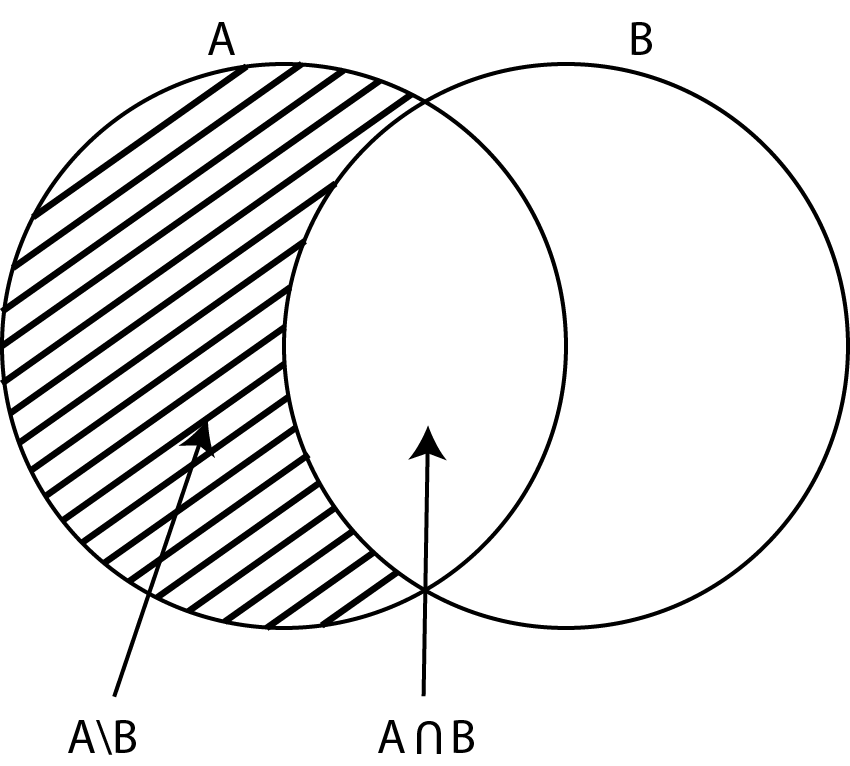
\includegraphics[width=0.5\linewidth]{chapter/sets and elements/intersection.png}
\end{center}


\begin{para}
    Note that $A\text{\\}B$ AND $B$ are disjoint i.e, $(A\text{\\}B) \cap B = \emptyset$
\end{para}

\begin{para}
    E.g: Using the previous example, with $A = \{1,2,3,4\}$, $B = \{3,4,5,6\}$ we have $A\text{\\}B$ = $\{1,2\}$
\end{para}


\subsection{Symmetric Difference}

\begin{para}
    The Symmetric difference of the sets $A$ and $B$, denoted by $A \oplus B$ is the set consisting of those elements which belong to $A$ or $B$, but not both i.e, $A \oplus B = (A \cup B)\text{\\}(A \cap B)$ or $A \oplus B = (A \text{\\}B)\nobreakspace U \nobreakspace(B\text{\\}A)$\\
    E.g: If $A=\{1,2,3,4\}$, $B=\{3,4,5,6\}$, $A \oplus B = (A \cup B)\text{\\}(A \cap B)$ $=\{1,2,3,4,5,6\} \text{\\}\{3,4\}$ $= \{1,2,5,6\}$
\end{para}

\subsection{Product Set or Cartesian Product}
\begin{para}
    An $n$-tuple is an ordered array on $n$ written $(x_1,x_2,\ldots,x_n)$
\end{para}
\begin{para}
    $(1,2), (0, 100), (a, b)$ are examples of 2-tuples, while $(1,1,1), (a,c,b), (2,1,2)$ are cases of 3-tuples.
\end{para}

\begin{para}
    let $A$ and $B$ be two sets. The product set or cartesian product of $A$ and $B$, denoted by $A \times B$ is a set of all possible 2-tuples $(a,b)$, where $a \in A$ and $b \in B$, i.e. $A \times B = \{(x,y): x \in A, y \in B\}$ e.g. \\
    let $A=\{1,2,3\}$ and $B=\{a,b\}$, Then \\
    $A \times B = \{(1,a),(1,b),(2,a),(2,b),(3,a),(3,b)\}$\\
    while\\
    $B \times A = \{(a,1),(a,2),(a,3),(b,1),(b,2),(b,3)\}$
\end{para}

